\subsubsection{Swarm EFI TII TCT data products}

\begin{verbatim}
import datetime
import matplotlib.pyplot as plt
import numpy as np
import pathlib
import os

import geospacelab.visualization.mpl.dashboards as dashboards

cwd = pathlib.Path(os.path.abspath(''))
file_dir_figure = cwd / 'figures'
file_dir_figure.mkdir(parents=True, exist_ok=True)
\end{verbatim}

\paragraph{Swarm EFI TII TCT 2Hz data}

\subparagraph{Overview with a long time span}

\begin{verbatim}
def test_swarm_EFI_TII_TCT02_overview():
    """Test Swarm EFI TII TCT02 data product
    
    """
    dt_fr = datetime.datetime(2015, 3, 17, 8, 0)
    dt_to = datetime.datetime(2015, 3, 17, 18, 0)

    db = dashboards.TSDashboard(
        dt_fr=dt_fr, dt_to=dt_to, figure_config={'figsize': (8, 12)},
        )

    ds = db.dock(datasource_contents=['esa_eo', 'swarm', 'advanced', 'efi_tct02'], sat_id='A', add_APEX=True,)

    panel_layouts = [
        [ds['v_i_H_x'], ds['v_i_V_x'], ds['v_i_H_y'], ds['v_i_V_z']],
        [ds['v_SC_N'], ds['v_SC_E'], ds['v_SC_C']],
        [ds['E_H_x'], ds['E_H_y'], ds['E_H_z']],
        [ds['E_V_x'], ds['E_V_y'], ds['E_V_z']],
        [ds['B_x'], ds['B_y'], ds['B_z']],
        [ds['v_i_CR_x'], ds['v_i_CR_y'], ds['v_i_CR_z']],
        [ds['QUALITY_FLAG_BIN_AUX'],],
        [ds['CALIB_FLAG_BIN_AUX'],],
    ]

    db.set_layout(panel_layouts=panel_layouts)
    db.draw()
    db.add_title(title='Swarm -{} EFI TII TCT02 Overview'.format(ds.sat_id), fontsize='medium', append_time=True)

    db.save_figure(
        file_dir=file_dir_figure, 
        file_name='example_EFI_TII_TCT02_Swarm -{}_overview'.format(ds.sat_id), 
        dpi=100, 
        append_time=False)
    db.show()
test_swarm_EFI_TII_TCT02_overview()
\end{verbatim}

\begin{verbatim}
Create a new figure: Figure(800x1200).
\end{verbatim}

\begin{verbatim}
Load IGRF coefficients ...
\end{verbatim}

\begin{verbatim}
Searching the data product "EFI_TCT02" with the version "latest" on the server...
The file [PosixPath('/data/afys -ionosphere/data/ESA/SWARM/Advanced/EFI_TII/TCT02/0401/Sat_A/2015/SW_EXPT_EFIA_TCT02_20150317T000000_20150317T235959_0401.cdf')] already exists: skip downloading.
/opt/anaconda3/envs/Swarm/lib/python3.12/site -packages/numpy/_core/numeric.py:476: RuntimeWarning: invalid value encountered in cast
  multiarray.copyto(res, fill_value, casting='unsafe')
\end{verbatim}

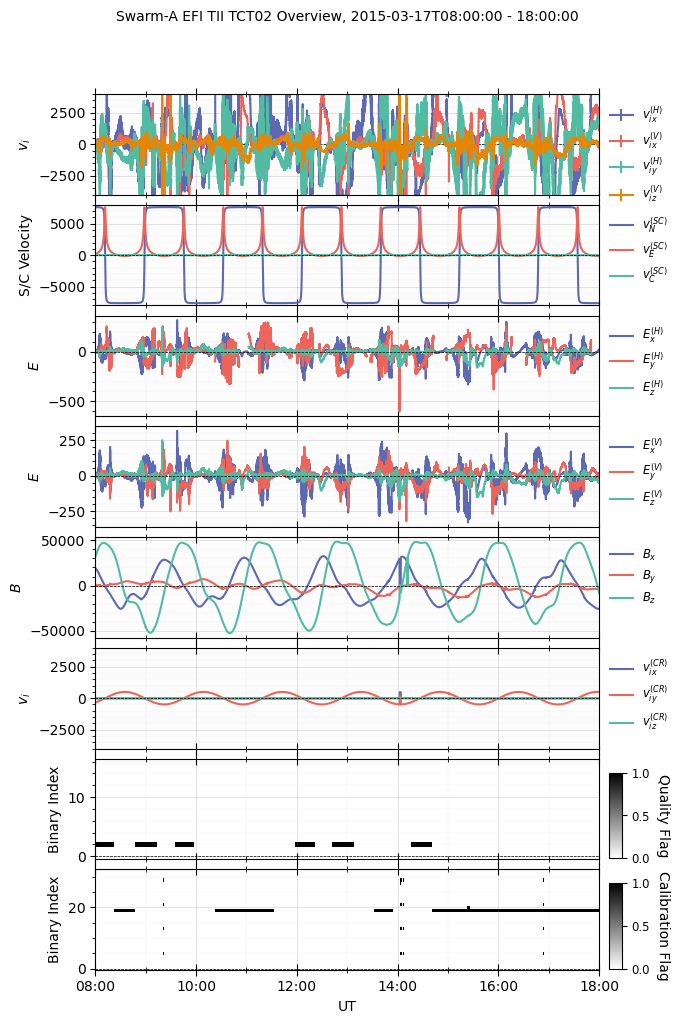
\includegraphics[width=0.7\linewidth]{files/f9b76a8bfab2158b755e845ae5b41e4f.png}

\subparagraph{Zoomed-in with a short time span}

\begin{verbatim}
def test_swarm_EFI_TII_TCT02_zoom():
    """Test Swarm EFI TII TCT02 data product
    
    """
    dt_fr = datetime.datetime(2015, 3, 17, 12, 40)
    dt_to = datetime.datetime(2015, 3, 17, 13, 10)

    db = dashboards.TSDashboard(
        dt_fr=dt_fr, dt_to=dt_to, figure_config={'figsize': (8, 12)},
        # timeline_extra_labels=['GEO_LAT', 'GEO_LON', 'APEX_LAT', 'APEX_LON', 'APEX_MLT',]  # Not applicable for very scattered data points like AEJ_PBS peaks
        )

    ds = db.dock(datasource_contents=['esa_eo', 'swarm', 'advanced', 'efi_tct02'], sat_id='A', add_APEX=True,)

    panel_layouts = [
        [ds['v_i_H_x'], ds['v_i_V_x'], ds['v_i_H_y'], ds['v_i_V_z']],
        [ds['v_SC_N'], ds['v_SC_E'], ds['v_SC_C']],
        [ds['E_H_x'], ds['E_H_y'], ds['E_H_z']],
        [ds['E_V_x'], ds['E_V_y'], ds['E_V_z']],
        [ds['B_x'], ds['B_y'], ds['B_z']],
        [ds['v_i_CR_x'], ds['v_i_CR_y'], ds['v_i_CR_z']],
        [ds['QUALITY_FLAG_BIN_AUX'],],
        [ds['CALIB_FLAG_BIN_AUX'],],
    ]

    db.set_layout(panel_layouts=panel_layouts)
    db.draw()
    db.add_title(title='Swarm -{} EFI TII TCT02 Zoom'.format(ds.sat_id), fontsize='medium', append_time=True)
    
    db.save_figure(
        file_dir=file_dir_figure, 
        file_name='example_EFI_TII_TCT02_Swarm -{}_zoom'.format(ds.sat_id), 
        dpi=100, 
        append_time=False)
    db.show()
test_swarm_EFI_TII_TCT02_zoom()
\end{verbatim}

\begin{verbatim}
Create a new figure: Figure(800x1200).
Searching the data product "EFI_TCT02" with the version "latest" on the server...
The file [PosixPath('/data/afys -ionosphere/data/ESA/SWARM/Advanced/EFI_TII/TCT02/0401/Sat_A/2015/SW_EXPT_EFIA_TCT02_20150317T000000_20150317T235959_0401.cdf')] already exists: skip downloading.
\end{verbatim}

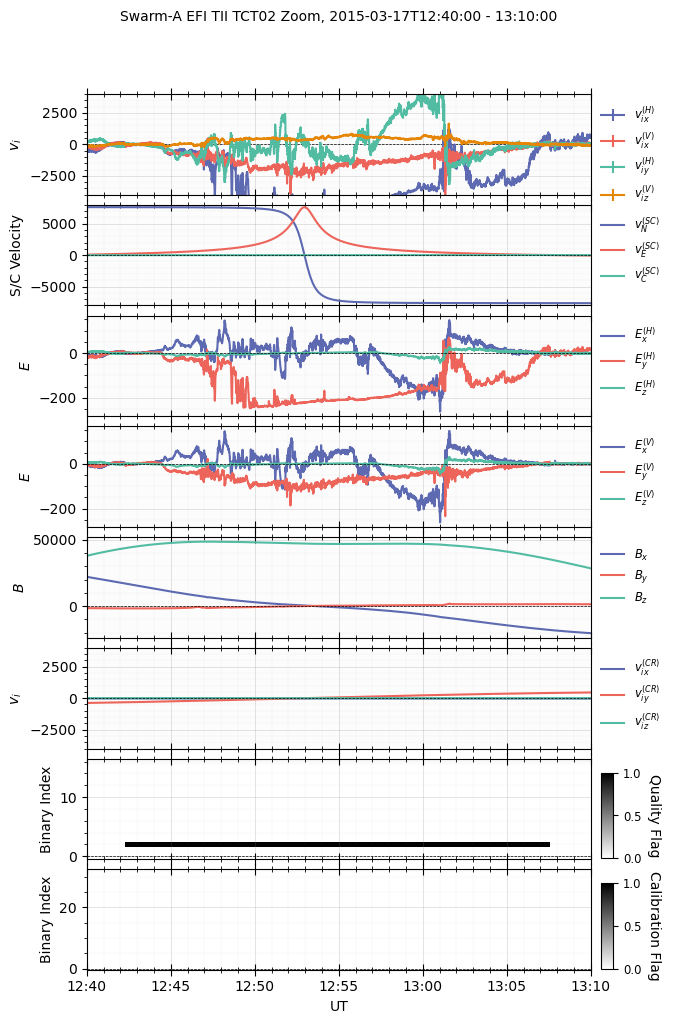
\includegraphics[width=0.7\linewidth]{files/2ba6d5416cf4759ee3511ffcecab9d58.png}

\paragraph{Swarm EFI TII TCT 16 Hz data}

\begin{verbatim}
def test_swarm_EFI_TII_TCT16_zoom():
    """Test Swarm EFI TII TCT16 data product
    
    """
    dt_fr = datetime.datetime(2015, 3, 17, 12, 40)
    dt_to = datetime.datetime(2015, 3, 17, 13, 10)

    db = dashboards.TSDashboard(
        dt_fr=dt_fr, dt_to=dt_to, figure_config={'figsize': (8, 12)},
        )

    ds = db.dock(datasource_contents=['esa_eo', 'swarm', 'advanced', 'efi_tct16'], sat_id='A', add_APEX=True,)

    panel_layouts = [
        [ds['v_i_H_x'], ds['v_i_V_x'], ds['v_i_H_y'], ds['v_i_V_z']],
        [ds['v_SC_N'], ds['v_SC_E'], ds['v_SC_C']],
        [ds['E_H_x'], ds['E_H_y'], ds['E_H_z']],
        [ds['E_V_x'], ds['E_V_y'], ds['E_V_z']],
        [ds['B_x'], ds['B_y'], ds['B_z']],
        [ds['v_i_CR_x'], ds['v_i_CR_y'], ds['v_i_CR_z']],
        [ds['QUALITY_FLAG_BIN_AUX'],],
        [ds['CALIB_FLAG_BIN_AUX'],],
    ]

    db.set_layout(panel_layouts=panel_layouts)
    db.draw()
    db.add_title(title='Swarm -{} EFI TII TCT16 Zoom'.format(ds.sat_id), fontsize='medium', append_time=True)

    db.save_figure(
        file_dir=file_dir_figure, 
        file_name='example_EFI_TII_TCT16_Swarm -{}_zoom'.format(ds.sat_id), 
        dpi=100, 
        append_time=False)
    db.show()
test_swarm_EFI_TII_TCT16_zoom()
\end{verbatim}

\begin{verbatim}
Create a new figure: Figure(800x1200).
Searching the data product "EFI_TCT16" with the version "latest" on the server...
INFO: Indexing the files for the product EFI_TCT16 of the satellite A ...
The file [PosixPath('/data/afys -ionosphere/data/ESA/SWARM/Advanced/EFI_TII/TCT16/0401/Sat_A/2015/SW_EXPT_EFIA_TCT16_20150317T000000_20150317T235959_0401.cdf')] already exists: skip downloading.
\end{verbatim}

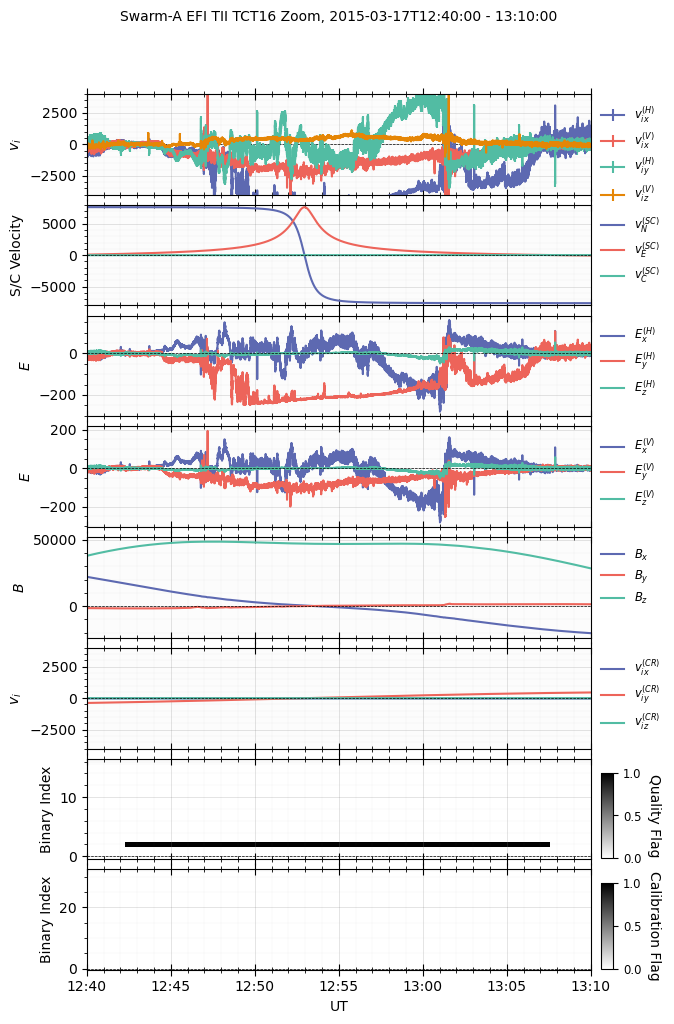
\includegraphics[width=0.7\linewidth]{files/aecc506c2c2541c2bb5e2a9264136729.png}